\documentclass{article}
\usepackage{microtype}
\usepackage{graphicx}
\usepackage{booktabs}
\usepackage{amsmath,amssymb}
\usepackage{hyperref}
\usepackage{url}

% ICML 2025 style used purely for formatting. No [accepted] option -> anonymous
% (author info is auto-removed). Venue notice below is overridden to neutral text.
\usepackage{icml2025}

% Neutralize the venue-specific submission notice and PDF metadata (no ICML branding).
\makeatletter
\renewcommand{\Notice@String}{Preliminary work. Under review. Please do not distribute.}
\makeatother
\hypersetup{pdfsubject={}, pdfauthor={Anonymous}, pdfkeywords={}}

\icmltitlerunning{How Low Can Chronos-2 Go? Post-Training Quantization of a TSFM}

\begin{document}

\twocolumn[
\icmltitle{How Low Can Chronos-2 Go? Post-Training Quantization\\
of a Time-Series Foundation Model}

% Anonymous submission: real author info omitted. The style renders
% "Anonymous Authors" / "Anonymous Institution" regardless of what appears here.
\begin{icmlauthorlist}
\icmlauthor{Anonymous Author}{anon}
\end{icmlauthorlist}

\icmlaffiliation{anon}{Anonymous Institution}
\icmlcorrespondingauthor{Anonymous Author}{anon@example.com}

\icmlkeywords{quantization, time-series foundation models, forecasting, model compression}

\vskip 0.3in
]

\printAffiliationsAndNotice{}

% Fill columns top-down; keep any slack at the column bottom instead of letting
% ICML's \flushbottom stretch inter-paragraph glue (which balloons list spacing).
\raggedbottom

\begin{abstract}
Time-series foundation models (TSFMs) such as Chronos-2 deliver strong zero-shot
probabilistic forecasts, but their deployment cost is rarely studied and, unlike large
language models, \emph{nothing} is known about how they respond to post-training
quantization (PTQ). We present the first systematic PTQ study of TSFMs: 39
weight-quantization configurations spanning seven method families (round-to-nearest,
torchao, bitsandbytes INT8/NF4, HQQ, GPTQ, GPTAQ, and activation-aware scale folding)
and two- to eight-bit precision, evaluated zero-shot on the 27-dataset Chronos benchmark
across four models and three architectures (encoder-only Chronos-2, encoder--decoder
Chronos-Bolt, decoder-only TimesFM-2.5). Beyond point (MASE) and probabilistic
(weighted quantile loss, WQL) accuracy, we introduce two calibration-aware
diagnostics---mean absolute coverage error and a quantile-crossing rate---because a
probabilistic forecaster can degrade in ways aggregate accuracy cannot see. Five
findings emerge. (i)~8-bit quantization is free for every method. (ii)~Hessian-aware
GPTQ retains full-precision accuracy down to \textbf{3 bits} (WQL retention 1.05), and
asymmetric-calibration GPTAQ extends the parity frontier (1.016); every PTQ method
collapses at 2 bits. (iii)~The \emph{method} matters far more than the \emph{bit-width}:
at 4 bits, retention spans 0.996--1.66. (iv)~Interval calibration and quantile
monotonicity degrade \emph{before} accuracy does---and we trace this damage
\emph{entirely} to the 3-linear quantile head: protecting 3.2\% of the weights
eliminates it at every bit-width, whereas accuracy damage is distributed across the
encoder. (v)~Two cheap repairs follow: post-hoc quantile sorting (free, provably never
worse) eliminates crossing, and split-conformal recalibration restores nominal coverage
for \emph{every} method at \emph{every} bit-width---even fp32 improves. We release the
framework, which reproduces published per-task benchmark numbers to $<\!10^{-6}$, and
all per-series predictions.
\end{abstract}

\section{Introduction}
Time-series foundation models (TSFMs)---Chronos \citep{chronos}, Chronos-2
\citep{chronos2}, TimesFM, Moirai---forecast unseen series zero-shot and are increasingly
deployed on CPU-only servers, edge devices, and high-throughput batch pipelines where
full-precision inference is costly. Quantization is the standard efficiency lever for
large language models (LLMs), but its lessons do not obviously transfer to TSFMs, which
are small (Chronos-2 has 120M parameters, a regime where quantization bites harder
\citep{qeval}), encoder-only and non-autoregressive (no KV cache, so LLM decode-centric
methods do not apply), and---critically---emit \emph{probabilistic} forecasts whose
calibration and quantile monotonicity matter, not just point accuracy.

Despite an extensive LLM-quantization literature, \textbf{no published work quantizes the
weights of any Chronos-family or comparable TSFM} (in that literature ``quantization''
usually denotes Chronos-1's input value-\emph{binning}, a distinct notion). We close that
gap with a controlled study across method families, bit-widths, and models, and argue
that evaluating a \emph{quantized probabilistic} forecaster demands metrics beyond those
on TSFM leaderboards.

\vspace{2pt}\noindent\textbf{Contributions.}
\begin{itemize}\itemsep2pt \topsep2pt \parskip0pt
\item The first systematic PTQ study of TSFMs: 39 configurations across 7 method
families, 5 bit-widths, and 4 models spanning 3 architectures (Chronos-2, Chronos-Bolt
small/base, TimesFM-2.5), zero-shot on 27 datasets with bootstrap confidence intervals
on every aggregate.
\item A calibration-aware evaluation protocol for compressed probabilistic forecasters,
adding interval-coverage error and a quantile-crossing rate, which reveal failure modes
invisible to WQL/MASE.
\item A \emph{mechanism}: module-family sensitivity and weight-space SNR diagnostics
showing calibration damage is gated exclusively by the 3-linear quantile head, while
accuracy damage is distributed.
\item Two mitigations with a deployment recipe: an fp32 head (prevention, 3.2\% of
weights) and post-hoc sorting + split-conformal recalibration (cure, at any bit-width).
\item An open framework that reproduces published benchmark numbers to floating-point
precision and releases all per-series predictions.
\end{itemize}

\section{Setup}
\textbf{Models.} Chronos-2 \citep{chronos2} (\texttt{amazon/chronos-2}) is a
119.5M-parameter, T5-derived \emph{encoder-only} transformer (12 layers,
$d_{\text{model}}{=}768$, RoPE, alternating ``time'' and ``group'' attention). It ingests
patches of a per-instance-normalized series through a residual embedding (no input
tokenization) and emits, in one non-autoregressive forward pass, direct multi-step
forecasts at 21 quantile levels. It ships in fp32 (478~MB). Quantization targets all 126
\texttt{nn.Linear} weights---including the patch embeddings and the 3-linear quantile
head (3.2\% of weights), except in arms that explicitly protect the head; LayerNorm
stays in fp32, and bf16 (not fp16, which overflows in T5-lineage models) is the
deployment baseline. As cross-model arms we also quantize Chronos-Bolt small/base
\citep{chronos} (48M/205M), \emph{encoder--decoder} T5 forecasters, through the same
harness (fp32 reproduces their published per-task numbers to 0.34\%/0.72\%; their
quantile head is protected by default), and TimesFM-2.5
(\texttt{google/timesfm-2.5-200m-pytorch}, 200M), a \emph{decoder-only} autoregressive
forecaster with a continuous quantile head, via a torch-only adapter (deterministic
single decode step at horizons $\le$56; head and tokenizer protected as in our
``+head'' arms). TimesFM-2.5 has no published per-task reference on this suite (we
sanity-anchor the adapter by its dev-subset skill exceeding Chronos-2's); its built-in
\texttt{fix\_quantile\_crossing} auto-sort is disabled in all arms so QCR is measured
honestly.

\vspace{2pt}\noindent\textbf{Methods.} We evaluate weight-only PTQ across seven families
runnable on commodity hardware: \textbf{RTN} (symmetric round-to-nearest,
per-channel/per-tensor, plus a simulated sub-8-bit sweep); \textbf{torchao} INT8
weight-only and INT8 dynamic-activation (W8A8); \textbf{bitsandbytes} LLM.int8()
\citep{llmint8} and NF4 \citep{qlora}; \textbf{HQQ} \citep{hqq}, a calibration-free
half-quadratic solver; \textbf{GPTQ} \citep{gptq}, a Hessian-aware error-compensating
quantizer implemented directly on the model's linear layers with one-shot calibration;
\textbf{GPTAQ} \citep{gptaq}, its asymmetric-calibration extension that corrects each
layer toward the \emph{full-precision} network's activations; and \textbf{AWQ-style}
activation-aware scale folding \citep{awq}. Methods are exercised at W8, W4 (group size
64/128), W3, and W2---39 full-benchmark configurations in total.

\vspace{2pt}\noindent\textbf{Protocol \& metrics.} We evaluate zero-shot on the
27-dataset Chronos benchmark \citep{chronos} (190{,}674 forecasts) using the \texttt{fev}
library---the harness the Chronos-2 authors use---so our numbers are directly comparable
with the public leaderboard. Point accuracy is MASE and probabilistic accuracy is
weighted quantile loss (WQL, 9 levels); our full-precision Chronos-2 attains 0.425 WQL
skill and an 88\% win rate over seasonal-naive, and our seasonal-naive matches the
published per-task MASE/WQL to $<\!10^{-6}$. The key quantity is \textbf{retention}: the
geometric-mean ratio $\mathrm{WQL}(\text{quant})/\mathrm{WQL}(\text{fp32})$ over the 27
tasks (1.00~=~parity), with a 1000-resample bootstrap 95\% CI. Because a probabilistic
forecaster can lose quality without moving WQL, we add two diagnostics. \textbf{MACE}
(mean absolute coverage error) averages $|\text{empirical}-\text{nominal}|$ over the
central 80/60/40/20\% intervals. \textbf{QCR} (quantile-crossing rate) is the fraction
of forecast points whose predicted quantiles are non-monotone. Two further protocols: a
\emph{module-family sensitivity} sweep (dev tier: 8-task subset) that partitions the 126
linears into six disjoint families, quantized or protected one family at a time; and an
offline \emph{repair} arm applying monotone rearrangement (quantile sorting)
\citep{rearrangement,fakoor} and 2-fold series-split conformal recalibration \citep{cqr}
to the persisted predictions of every full-tier arm.

\section{Results}
Table~\ref{tab:main} summarizes representative configurations; Fig.~\ref{fig:main} plots
the accuracy--bit curve and calibration. The complete 39-variant matrix is released.

\begin{table}[t]
\centering\small
\setlength{\tabcolsep}{1.6pt}
\renewcommand{\arraystretch}{1.05}
\caption{Representative variants, full 27-task benchmark. Retention = geometric-mean
WQL(quant)/WQL(fp32), [95\% bootstrap CI]. \emph{c80} = empirical coverage of the
nominal-80\% interval (fp32: 0.750). \emph{QCR} = quantile-crossing rate (fp32: 0.039).
BPW = effective bits/weight incl.\ scales; $\dagger$ accuracy-exact simulation
(dequantized grid in fp32)---BPW is the \emph{achievable} footprint. ``+head'' = all
linears quantized except the 3-linear quantile head (kept fp32).}
\label{tab:main}
\begin{tabular}{@{}lcccccc@{}}
\toprule
Variant & Bits & BPW & WQL ret.\ [CI] & MASE & c80 & QCR \\
\midrule
fp32 (ref)    & 32 & 32.0        & 1.000              & 1.000 & .750 & .039 \\
RTN W8        & 8  & 8.03        & 0.999 [.997,1.00]  & 1.001 & .749 & .149 \\
GPTQ W8       & 8  & 8.13$\dagger$ & 1.000 [.990,1.01] & 1.003 & .749 & .064 \\
HQQ W8        & 8  & 9.00        & 1.002 [1.00,1.00]  & 1.000 & .746 & .086 \\
\textbf{RTN W8+head} & 8 & 8.03  & \textbf{0.999 [.998,1.00]} & 1.000 & .751 & .037 \\
\textbf{GPTQ W4}& 4 & 4.13$\dagger$ & \textbf{1.002 [.985,1.02]} & 1.011 & .756 & .254 \\
GPTAQ W4      & 4  & 4.25$\dagger$ & 1.000 [.987,1.01] & 1.008 & .745 & .226 \\
HQQ W4        & 4  & 5.00        & 1.060 [1.02,1.12]  & 1.027 & .630 & .420 \\
NF4 W4        & 4  & 4.13        & 1.065 [1.00,1.15]  & 1.026 & .686 & .396 \\
HQQ W4+head   & 4  & 5.00        & 1.020 [.985,1.06]  & 1.016 & .751 & .021 \\
NF4 W4+head   & 4  & 4.13        & 1.045 [.984,1.13]  & 1.025 & .761 & .022 \\
AWQ W4        & 4  & 4.03$\dagger$ & 1.639 [1.38,2.01] & 1.409 & .481 & .599 \\
GPTQ W3       & 3  & 3.25$\dagger$ & 1.047 [.988,1.14] & 1.059 & .791 & .366 \\
\textbf{GPTAQ W3}& 3 & 3.25$\dagger$ & \textbf{1.016 [.988,1.05]} & 1.034 & .770 & .379 \\
HQQ W3        & 3  & 4.20        & 1.229 [1.09,1.48]  & 1.143 & .666 & .589 \\
GPTAQ W2      & 2  & 2.25$\dagger$ & 1.937 [1.55,2.48] & 1.816 & .642 & .833 \\
RTN W2        & 2  & 2.0$\dagger$  & 4.082 [3.08,5.57] & 3.108 & .060 & .523 \\
\bottomrule
\end{tabular}
\end{table}

\begin{figure*}[t]
\centering
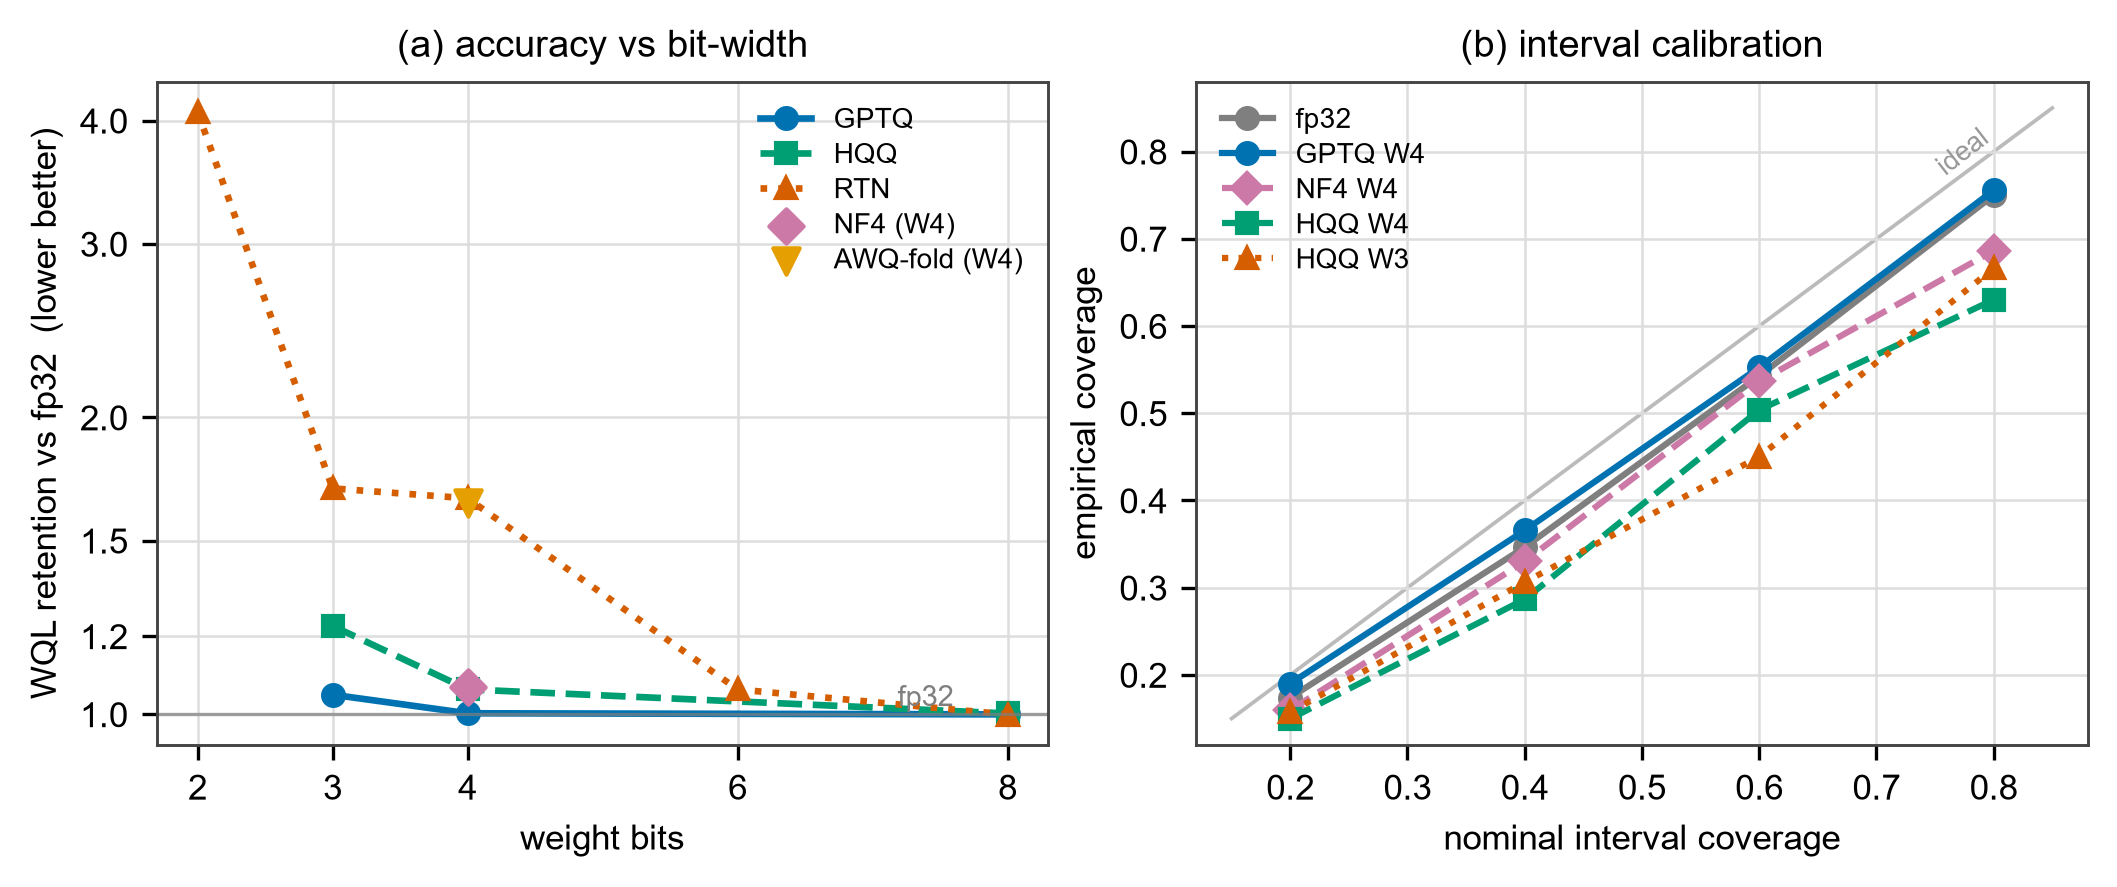
\includegraphics[width=0.84\textwidth]{figures/fig1_accuracy_calibration.png}
\caption{\emph{(a)} WQL retention vs weight bits by method (log scale; lower is better,
1.0~=~fp32). GPTQ tracks fp32 to 3 bits; the method spread at 4 bits exceeds the
8$\to$4-bit gap of any single method; AWQ-fold sits on the RTN line. \emph{(b)} Empirical
vs nominal interval coverage: GPTQ-W4 tracks fp32 while HQQ/NF4 systematically
under-cover.}
\label{fig:main}
\end{figure*}

\vspace{2pt}\noindent\textbf{F1---8-bit is free, for every method.} All six W8
configurations retain WQL within $[0.999,1.013]$ and MASE within $[1.000,1.011]$ of fp32
(Table~\ref{tab:main}; Fig.~\ref{fig:main}a), at $4\times$ compression. Even W8A8 with
dynamic-activation quantization costs only 1.3\%. Eight-bit quantization of Chronos-2
is, for practical purposes, lossless regardless of method.

\vspace{2pt}\noindent\textbf{F2---error-compensating PTQ reaches full precision at 3
bits; everything collapses at 2.} GPTQ retains parity at 4 bits (retention 1.00, both
group sizes) and at \textbf{3 bits} (1.047, CI $[0.988,1.137]$---statistically
indistinguishable from fp32), where HQQ loses 23\% and naive RTN 70\%
(Fig.~\ref{fig:main}a). GPTAQ extends the frontier: W3 retention
\textbf{1.016} $[0.988,1.053]$ and W4 parity (1.000). Its asymmetry strength matters:
the official $\alpha{=}0.25$ beats $\alpha{=}1.0$ (1.016 vs 1.087 at W3). At 2 bits
every PTQ method collapses---GPTAQ 1.94, GPTQ 2.17, RTN-sim 4.08---so sub-3-bit
deployment needs quantization-aware training (future work). (A dev-subset signal that
GPTQ \emph{beat} fp32 resolved to parity at full scale; we report the confirmed
result.)

\vspace{2pt}\noindent\textbf{F3---method dominates bit-width.} At a fixed 4 bits, WQL
retention spans 0.996 (GPTQ) to 1.66 (RTN)---a 66-point gap---whereas moving a
\emph{good} method from 8 to 4 bits costs $\le$6\% (Fig.~\ref{fig:main}a). For a TSFM,
\emph{how} you quantize matters far more than \emph{how much}, inverting the intuition
that bit-width is the primary knob.

\vspace{2pt}\noindent\textbf{F4---calibration degrades before accuracy, and the quantile
head is the entire mechanism.} At 8 bits, accuracy is perfectly retained yet the
quantile-crossing rate already quadruples ($0.039\to0.149$ for RTN)---a defect WQL and
MASE cannot see; at 4 bits HQQ and NF4 sag to c80 0.630/0.686 (a nominal ``80\%'' band
that holds 63\%) while GPTQ keeps 0.756. Sensitivity experiments explain \emph{why}.
Partitioning the 126 linears into disjoint families (dev tier, W4 RTN-sim): quantizing
\emph{only} the 3-linear quantile head---3.2\% of weights---reproduces the full collapse
(WQL 2.115, vs 2.130 with all 126 quantized), while protecting only the head recovers to
1.143 with \emph{better-than-fp32} calibration (c80 0.778, QCR 0.002). Accuracy damage
is instead distributed (only-group-attention 1.001, only-FFN 1.086), and
first/last-block-protection folklore does not hold here. Full-benchmark confirmation
(Table~\ref{tab:main}, ``+head''): an fp32 head returns W8-RTN's QCR to 0.037 (fp32:
0.039)---the F4 quadrupling is \emph{entirely} head-gated---and repairs W4 coverage:
HQQ 0.630$\to$0.751 (WQL 1.020), NF4 0.686$\to$0.761 (1.045), at a cost of
$\approx$11--13~MB. Accuracy-only evaluation therefore overstates a compressed
forecaster's quality \citep{accuracy}---but prevention costs 3\% of the weight budget.

\vspace{2pt}\noindent\textbf{F5---damage is tail-concentrated.} Mean retention hides
worst cases: HQQ-W3 averages 1.23 but its worst task is $8.2\times$ and 44\% of tasks
exceed 1.10; GPTQ-W4 has a median per-task ratio of 0.998 and only 4\% of tasks above
1.10. Per-series distributions---released for every run---are the honest picture.

\vspace{2pt}\noindent\textbf{F6---no LLM-style outliers: the head fails on weight-space
SNR, explaining the AWQ negative result.} For Chronos-2 the AWQ scale fold is
\emph{exact} (we verify the fold numerically)---yet AWQ-fold+RTN
at 4 bits (1.64) barely differs from plain RTN (1.66) and is far behind GPTQ. Activation
diagnostics show why: Chronos-2 has \emph{no} massive-magnitude activation outliers
(global $|x|_{\max}\!\approx\!11$; the fraction of channels exceeding $|x|{>}6$ is zero
in most layers and at most 1.6\%), only ReLU-sparsity channel heterogeneity (per-channel
kurtosis is modest; pooled kurtosis is inflated by dead channels). The head's failure is
instead a weight-space signal-to-noise problem: at W4 its output layer's relative
reconstruction error is 7.83---quantization noise $\approx8\times$ the output
signal, over $100\times$ any other linear (all $<0.07$)---because small quantile
differences ride on large weights with no downstream layer to compensate. Activation
\emph{scaling} cannot fix a weight-space SNR deficit; Hessian-aware \emph{compensation}
(GPTQ/GPTAQ) can.

\vspace{2pt}\noindent\textbf{F7---post-hoc repairs: sorting is free; conformal restores
coverage everywhere.} Sorting predicted quantiles (monotone rearrangement) provably
never increases quantile loss \citep{rearrangement,fakoor}; empirically it zeroes QCR
for \emph{every} arm at never-worse WQL, and even recovers accuracy where crossing is
severe (HQQ-W3 $1.229\to1.170$). Coverage is only partially restored (HQQ-W4 c80
$0.630\to0.703$): crossing is cosmetic damage; the residual under-coverage is genuine
distributional corruption. Split-conformal recalibration (2-fold series split,
sort-before-calibrate) fixes that: c80 returns to 0.78--0.80 for every method at every
bit-width, from RTN-W2-sim ($0.060\to0.782$) to AWQ-W3 ($0.480\to0.795$)---and raw fp32
itself under-covers (0.750; MACE $0.059\to0.017$ conformal), so a
quantized-and-recalibrated model is better calibrated than the raw fp32 reference.
Conformal retention is reported against the conformalized fp32 (same stage), leaving
accuracy essentially unchanged. TimesFM-2.5 supplies independent evidence that this
repair is a general TSFM need rather than a quantization artifact: with its auto-sort
disabled, its \emph{fp32} model already emits crossed quantiles (QCR 0.109, c80
0.709)---the vendor ships exactly this sorting repair, on by default. Caveat: the
conformal guarantee is series-level (residuals pooled across horizons), not per-horizon.

\vspace{2pt}\noindent\textbf{F8---the findings transfer across architectures.} On
encoder--decoder Chronos-Bolt small (48M) and base (205M), with the quantile head
protected by default, \emph{every} method is at parity: small W4-HQQ 0.994 and W3-GPTQ
0.986; base 0.9997--1.005 across all arms; calibration untouched (base c80 0.782 = fp32,
QCR unchanged). On decoder-only TimesFM-2.5, likewise head-protected, W8-RTN 0.998,
W4-GPTQ 0.999 $[0.950,1.034]$, and W4-HQQ 1.009 are at parity, while W3-GPTQ degrades
(1.101 $[1.054,1.155]$)---its accuracy cliff sits one bit higher than Chronos-2's, a
genuine cross-model difference. Calibration is again untouched in every arm (c80
0.686--0.715 vs fp32's 0.709; QCR 0.097--0.115 vs 0.109)---third-architecture
confirmation of the head mechanism.

\vspace{2pt}\noindent\textbf{Efficiency.} Storage-real 4-bit models occupy $\approx$60~MB
($8\times$ smaller) and cut peak batch-1 GPU memory from 493~MB (fp32) to 87~MB for NF4
($5.7\times$; Table~\ref{tab:eff}). Throughput is flat ($\sim$120 series/s at batch 256,
vs 110 for fp32): our reference dequantize-then-GEMM paths buy footprint, not speed.
Memory-bound and edge deployments benefit immediately.

\begin{table}[t]
\centering\small
\setlength{\tabcolsep}{5pt}
\renewcommand{\arraystretch}{1.05}
\caption{Inference efficiency (storage-real variants, NVIDIA RTX 2000 Ada laptop, context
2048, horizon 64). Peak memory and latency at batch 1; throughput at batch 256.}
\label{tab:eff}
\begin{tabular}{@{}lcccc@{}}
\toprule
Model & Size MB & Peak GPU MB & Lat.\ ms & Thr.\ ser./s \\
\midrule
fp32       & 478 & 493 & 30 & 110 \\
INT8 (HQQ) & 120 & 176 & 42 & 122 \\
NF4 (W4)   & 60  & 87  & 45 & 120 \\
\bottomrule
\end{tabular}
\end{table}

\section{Discussion, Limitations, Conclusion}
\textbf{Recommendation.} (a)~At 8 bits use any toolkit, but keep the 3-linear quantile
head in fp32 (retention 0.9995 with fp32-level calibration). (b)~For 4--3 bits use GPTQ
or GPTAQ (GPTAQ-W3 1.016); below 3 bits PTQ collapses---use QAT. (c)~Always sort
predicted quantiles post-hoc: it is free, provably never worse, and zeroes quantile
crossing. (d)~When calibrated intervals matter, wrap the deployed model in
split-conformal recalibration: it restores nominal coverage at any bit-width and even
improves fp32. Report calibration and quantile-crossing alongside WQL whenever a
probabilistic model is compressed.

\vspace{2pt}\noindent\textbf{Limitations.} We study univariate zero-shot tasks;
covariate/multivariate tasks and quantization-aware training (the indicated sub-3-bit
path) are future work. Module-family sensitivity numbers are dev-tier (8 tasks).
GPTQ/GPTAQ/AWQ arms are accuracy-exact simulations; realized speed needs packed kernels
we do not implement (achievable footprints reported). Latency is hardware-specific;
retention ratios are the transferable claim. Conformal guarantees are series-level,
pooled across horizons.
We assess but exclude KV-cache/vector methods such as TurboQuant \citep{turboquant},
which do not apply to a cache-free encoder.

\vspace{2pt}\noindent\textbf{Conclusion.} Across three architectures, TSFMs quantize
remarkably well: 8-bit is free and error-compensating PTQ holds full-precision accuracy
to 3--4 bits. The
failure mode that does appear---calibration and monotonicity degrading before
accuracy---is gated by 3.2\% of the weights (the quantile head) and is preventable at
the source (fp32 head) or curable post hoc (sorting + split-conformal) at any bit-width.
Compressing a probabilistic forecaster is not merely an accuracy-retention problem---but
with the head protected and quantiles recalibrated, it is close to a solved one down to
3 bits. Code and all per-series predictions are released.

\bibliography{refs}
\bibliographystyle{icml2025}

\end{document}
